\documentclass[10pt]{article}
\usepackage[margin=0.62in,top=0.5in,bottom=0.5in]{geometry}
\usepackage{amsmath,amssymb}
\usepackage{graphicx}
\usepackage{microtype}
\usepackage[T1]{fontenc}
\usepackage{newtxtext,newtxmath}
\usepackage[dvipsnames]{xcolor}
\usepackage{enumitem}
\setlist[itemize]{leftmargin=1.1em,itemsep=2pt,topsep=3pt,parsep=0pt}
\pagestyle{empty}
\setlength{\parindent}{0pt}
\setlength{\parskip}{3pt}

\newcommand{\proj}[1]{\texttt{#1}}

\begin{document}

{\large\bfseries The \proj{proj0}/\proj{proj5} spectral ratio is projection shear, in closed form}

Cail Daley (CEA Paris-Saclay) \hfill 18 August 2026

\vspace{2pt}\hrule\vspace{6pt}

Tom's \proj{proj0}/\proj{proj5} ratio is predicted, with no free parameters, by the local Jacobian of SFL relative to ZEA over the 1500d footprint and the Planck 2018 lensed $C_\ell$: few-percent agreement in TT and EE from $\ell\simeq1000$ to $4000$, with the acoustic structure coming out of the model rather than being put into it.

\begin{center}
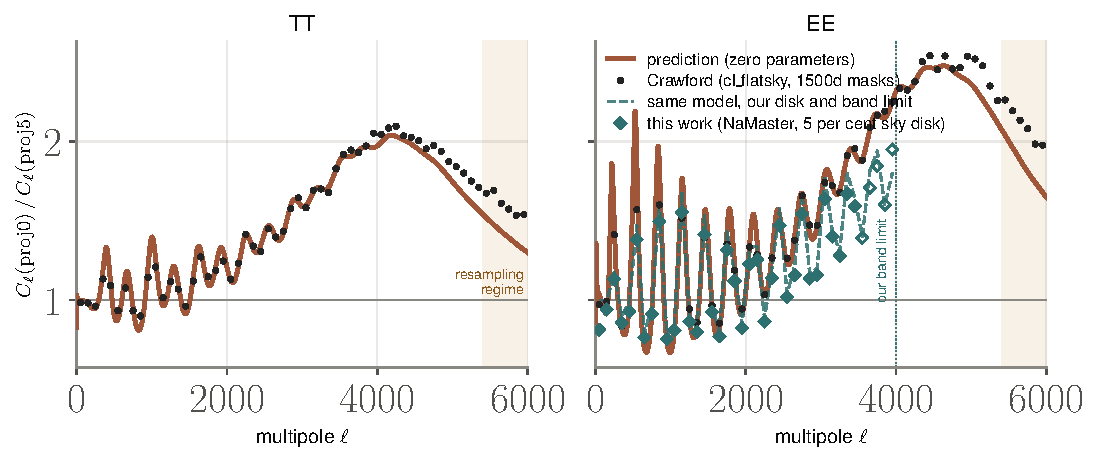
\includegraphics[width=0.8\textwidth]{onepager_ratio.pdf}
\end{center}

{\footnotesize\setlength{\parskip}{2pt}
\textbf{Figure.} Black: Tom's measured full-mask ratio (one realization --- his pickles are shaped $(4,60)$, but rows 1--3 are identically zero).
Orange: the prediction, unbinned, from his real apodization mask, the lensed Planck 2018 spectrum, and his band limit $\ell=7999$.
His ``EE'' is the EE spectrum run through the same scalar machinery as TT, so both panels test the scalar relation.
Nothing is divided by a transfer function: pixel windows cancel in the ratio.
\par}

\vspace{2pt}\hrule\vspace{2pt}

\textbf{Where the curve comes from.}
Reprojection is smooth, so over any small patch it acts as a linear map with Jacobian $J$ --- here the Jacobian of \proj{proj0} coordinates with respect to \proj{proj5} coordinates, at that point of the sky.
Let $C(\boldsymbol\ell)$ be the two-dimensional flat-sky power spectrum, $\boldsymbol\ell=(\ell_x,\ell_y)$; the familiar $C_\ell$ is its average over annuli of fixed $\ell=|\boldsymbol\ell|$.
A linear remap of the map relabels its Fourier modes, so the 2D spectrum transforms exactly:
\[
C_{\text{\proj{proj0}}}(\boldsymbol\ell) \;=\; |\det J|\; C_{\text{\proj{proj5}}}\!\left(J^{\mathsf T}\boldsymbol\ell\right).
\]
$J$ has two principal stretch factors, its singular values $s_1\ge s_2$; from them define the shear $g=(s_1-s_2)/(s_1+s_2)$ and the magnification $\mu=s_1 s_2=|\det J|$ ($=1$ here to machine precision: SFL and ZEA are both equal-area).
Let $\chi$ be the azimuth of $\boldsymbol\ell$ measured from $J$'s first principal axis --- with the axes aligned to the grid, $\tan\chi=\ell_y/\ell_x$ --- so annulus binning is a uniform average over $\chi$.
Averaging additionally over the footprint, weighted by the squared apodization mask $W^2$ as a pseudo-$C_\ell$ estimator does, the predicted ratio is
\[
\frac{C_\ell(\text{\proj{proj0}})}{C_\ell(\text{\proj{proj5}})}
=\Big\langle\, \mu\,\frac{C\!\left(\ell\, r(\chi)\right)}{C(\ell)} \,\Big\rangle_{\chi,\,W^2},
\qquad
r(\chi)=\sqrt{s_1^2\cos^2\chi + s_2^2\sin^2\chi},
\]
where $C(\ell)$ is the input (sky) spectrum and $\ell\,r(\chi)=|J^{\mathsf T}\boldsymbol\ell|$ is the sky wavenumber that grid mode $\boldsymbol\ell$ actually samples.
Expanding for a spectrum that is locally a power law with logarithmic slope $n = \mathrm{d}\ln C/\mathrm{d}\ln\ell$, and comparing equal-area projections, gives the compact form
\[
\frac{C_\ell(\text{\proj{proj0}})}{C_\ell(\text{\proj{proj5}})}
\;=\;1+\frac{n(n+2)}{4}\,\langle g^2\rangle + \mathcal{O}(g^4).
\]
The term linear in $g$ averages away over $\chi$, so the effect is \emph{quadratic} in shear --- but not small: on the damping tail $n\approx-9$ gives $n(n+2)/4\approx16$, and the 1500d footprint's $\langle g^2\rangle=0.0442$ becomes an order-unity distortion (TT and EE differ only through their local slopes).
Evaluated with the true $C(\ell)$ rather than a power law, the prediction inherits the acoustic structure --- dips where a peak flattens the slope, rises where the tail steepens --- the part of the agreement that cannot be tuned.
Nothing is fitted: $J$ from the projection definitions, $C(\ell)$ from Planck 2018, the footprint from the real SPT-3G mask.

\vspace{2pt}
\textbf{Accounting for the whole measurement.}
Everything in Tom's runs --- the curve above and the two ways the data depart from it --- comes down to three mechanisms, none fitted.
\begin{itemize}
\item \emph{The ratio itself is geometry.}
On the full mask, measured/predicted stays within $3.3\%$ at every bandpower from $\ell=1050$ to $4050$, in both TT and EE.
\item \emph{His mask-variant runs fall below the curve because of the estimator, not the projection.}
Alongside the full mask, Tom repeated the measurement on two modified masks --- one with a corner cut away, one isotropically shrunk to the same area --- to test whether the excess was a mask effect.
Both variants are made by zeroing pixels outright, which leaves a hard edge, and \proj{cl\_flatsky} corrects only by $\langle W^2\rangle$ with no mode decoupling --- so those runs sit $15$--$25\%$ below the geometry above $\ell=4000$.
Convolving the prediction with the mask's exact coupling kernel closes the gap (TT at $\ell=4050$: $0.808\to0.996$ and $0.806\to0.976$) while moving the apodized full mask, the control, by under $1\%$.
A decoupled estimator (NaMaster) would not show this deficit at all.
\item \emph{His points rise above the curve at $\ell\gtrsim4500$ because of nearest-neighbour resampling.}
This excess is additive, not multiplicative --- flat in $C_\ell$ while the spectrum falls a decade beneath it --- and its amplitude scales as pixel$^{2.9}$; extrapolated from coarser grids to his $0.25'$, it predicts $1.009$--$1.124$ over $\ell=4050$--$5550$ against his measured $1.026$--$1.146$.
\end{itemize}

\vspace{8pt}

{\large\bfseries Reading the working-group notes through this lens}

\vspace{2pt}\hrule\vspace{6pt}

Several entries in the secondaries-call notes have been circling this question; we comment on them below.

\vspace{2pt}
\textbf{2025-11-10 (Winter 5yr, Marco).}
\emph{``It makes sense to produce the maps in \proj{proj0} but if you compute PS in \proj{proj0} you get incorrect results.''}
--- The formula says how incorrect, per multipole.
The size of the error is $\tfrac{1}{4}n(n+2)\langle g^2\rangle$ at leading order: percent-level where the spectrum is shallow, order-unity on the damping tail where $n\to-9$.
It is a scalar-convexity effect, so it applies to any spectrum computed on a sheared grid, TT included.

\vspace{2pt}
\textbf{2025-12-15.}
\emph{``Instead of using the theory spectrum, use the measured spectrum from CMB projected on \proj{proj0}''} / \emph{``using the sim-based Cls as the theory now to capture the projection effects.''}
--- That workaround \emph{is} the forward model, obtained empirically.
The expression above computes the same object analytically, from the footprint and the input spectrum, with no sims.
It also explains a follow-on observation, 2026-03-02: \emph{``depended quite a lot on the spectrum -- especially the CMB spectra, but the other components were ok.''}
The distortion depends on the spectrum only through its local slope, and $n(n+2)/4$ is steeply nonlinear in $n$: tSZ and foreground spectra have gentle slopes and barely move, while the CMB damping tail is the one place $n$ grows large enough to matter.
That the CMB is the component that misbehaves follows from the coefficient.

\vspace{2pt}
\textbf{2026-06-22.}
\emph{``if you go \proj{proj5}$\to$Cl\_a$\to$\proj{proj0}$\to$Cl\_b; Cl\_a/Cl\_b$\sim$2''} (hedged, ``maybe at high-$\ell$'').
--- For the 1500d footprint the predicted ratio reaches $\approx2$ by $\ell\simeq4000$--$4500$ and turns over above it; the figure on page 1 shows the full curve.
The hedge was well placed: it is a high-$\ell$ effect, and below $\ell\sim2000$ it is a few percent.

\vspace{2pt}
\textbf{2026-03-16 (unit test, Dhayaa).}
\emph{``start by making healpix $\to$ \proj{proj5} $\to$ healpix \ldots{} No issues here \ldots{} What if you multiply by beam? We get slightly different results.''}
--- Both halves are expected.
The clean round trip is the statement that reprojection is invertible geometry: whatever $J$ does one way it undoes the other.
The beam breaks it because a beam is applied \emph{in the grid frame}: an isotropic $B(\ell)$ imposed on the \proj{proj0} grid is $B(|J^{\mathsf T}\boldsymbol\ell|)$ on the sky --- an effective beam that is elliptical and position-dependent, with axis ratio $s_1/s_2$ set by the same Jacobian, computable in closed form from quantities already in hand.
It also answers 2025-06-10 (Marco), \emph{``Should I apply beam in \proj{proj5}? For the sims, it does not matter''}: it does matter, and the same expression says by how much.

\vspace{6pt}\hrule\vspace{3pt}
{\footnotesize This builds on the 2020--21 study begun with Caterina Umilt\`a, who built the original NaMaster analysis including the measurements overlaid here, and Gil Holder, who advised that work.
The recent analysis and derivations were developed jointly with Claude (Anthropic): CD --- conception, direction, validation; Claude --- the closed forms and the drafting of this note.\par}

\end{document}
